\section{Evaluation of Standard Strategies}
\label{sec:eval-common-strategies}

In order to construct new baselines and their performance differences,
we evaluated tiebreaking strategies for domain-independent optimal
classical planning.  In our experiments, the planners are based on Fast
Downward (revision 6251), and all experiments are run with a 5-minute,
2GB memory limit for the search binary (FD translation/preprocessing
times are not included in the 5-minute limit).  All experiments were
conducted on Xeon E5410@2.33GHz CPUs.  We used 1104 instances from 35
standard benchmark domains.

We first compared two commonly used tiebreaking strategies, $[f,h,\fifo]$, $[f,h,\lifo]$, which
first break ties according to $h$, and then apply \fifo or \lifo
last-resort tiebreaking, respectively.
Results for LMcut heuristic \cite{Helmert2009} and M\&S heuristic \cite{HelmertHHN14} are
shown in \reftbl{tbl:lmcut-ipc-full} and \reftbl{tbl:mands-ipc-full}
(leftmost 2 columns), respectively.
Differences in coverage are observed in several domains, and
$[f,h,\lifo]$ outperforms $[f,h,\fifo]$ overall.

\begin{table}[htbp]
 {
 \centering
 \begin{tabular}{|*{5}{c|}}
\hline
 & \multicolumn{4}{|c|}{Coverages (\# problems solved)} \\
\hline                                    
 Domain                                 &  $[f,h,\fifo]$ &  $[f,h,\lifo]$ &  $[f,\fifo]$ &  $[f,\lifo]$ \\ \hline
 sum(1104)                              &558             &\textbf{565}    &442           &556           \\ \hline
 {\relsize{-1}airport(50)}              &\textbf{27}     &26              &18            &26            \\
 % {\relsize{-1}barman-opt11(20)}         &0               &0               &0             &0             \\
 {\relsize{-1}blocks(35)}               &\textbf{28}     &\textbf{28}     &26            &26            \\
 {\relsize{-1}cybersec(19)}             &2               &\textbf{3}      &0             &\textbf{3}    \\
 {\relsize{-1}depot(22)}                &\textbf{6}      &\textbf{6}      &5             &5             \\
 {\relsize{-1}driverlog(20)}            &13              &13              &12            &13            \\
 {\relsize{-1}elevators-opt11(20)}      &15              &15              &14            &15            \\
 % {\relsize{-1}floortile-opt11(20)}      &6               &6               &6             &6             \\
 {\relsize{-1}freecell(80)}             &9               &9               &8             &9             \\
 % {\relsize{-1}grid(5)}                  &1               &1               &1             &1             \\
 % {\relsize{-1}gripper(20)}              &6               &6               &6             &6             \\
 % {\relsize{-1}hanoi(30)}                &12              &12              &12            &12            \\
 {\relsize{-1}logistics00(28)}          &\textbf{20}     &\textbf{20}     &16            &18            \\
 {\relsize{-1}miconic(150)}             &\textbf{140}    &\textbf{140}    &68            &\textbf{140}  \\
 {\relsize{-1}mprime(35)}               &21              &21              &19            &\textbf{22}   \\
 {\relsize{-1}mystery(30)}              &15              &16              &15            &15            \\
 {\relsize{-1}nomystery-opt11(20)}      &\textbf{14}     &\textbf{14}     &12            &13            \\
 {\relsize{-1}openstacks-opt11(20)}     &11              &\textbf{18}     &11            &\textbf{18}   \\
 {\relsize{-1}parcprinter-opt11(20)}    &13              &13              &12            &13            \\
 % {\relsize{-1}parking-opt11(20)}        &1               &1               &1             &1             \\
 {\relsize{-1}pathways(30)}             &5               &5               &4             &5             \\
 % {\relsize{-1}pegsol-opt11(20)}         &17              &17              &17            &17            \\
 {\relsize{-1}pipesworld-notankage(50)} &\textbf{15}     &14              &13            &13            \\
 {\relsize{-1}pipesworld-tankage(50)}   &8               &8               &7             &8             \\
 % {\relsize{-1}psr-small(50)}            &48              &48              &48            &48            \\
 % {\relsize{-1}rovers(40)}               &7               &7               &7             &7             \\
 {\relsize{-1}scanalyzer-opt11(20)}     &\textbf{10}     &\textbf{10}     &4             &\textbf{10}   \\
 % {\relsize{-1}sokoban-opt11(20)}        &19              &19              &19            &19            \\
 % {\relsize{-1}storage(30)}              &14              &14              &14            &14            \\
 {\relsize{-1}tidybot-opt11(20)}        &12              &12              &11            &11            \\
 % {\relsize{-1}tpp(30)}                  &6               &6               &6             &6             \\
 % {\relsize{-1}transport-opt11(20)}      &6               &6               &6             &6             \\
 {\relsize{-1}visitall-opt11(20)}       &10              &10              &9             &10            \\
 {\relsize{-1}woodworking-opt11(20)}    &\textbf{10}     &\textbf{10}     &6             &9             \\
 {\relsize{-1}zenotravel(20)}           &\textbf{11}     &\textbf{11}     &9             &\textbf{11}   \\\hline
\end{tabular}

 \caption{
 Coverage comparison (the number of instances solved in 5min, 2GB, LMcut
 heuristics) between
 the standard baseline tiebreaking algorithms. We highlight the
 best results when the difference between the maximum and the mininum coverage exceeds 2.
 }
 \label{tbl:lmcut-ipc-full}
 }
\end{table}

\begin{table}[htbp]
 {
 \centering
 \begin{tabular}{|*{5}{c|}}
\hline
                                        & \multicolumn{4}{|c|}{Coverages (\# problems solved)}  \\ \hline                                    
 Domain                                 &  $[f,h,\fifo]$ &  $[f,h,\lifo]$ &  $[f,\fifo]$ &  $[f,\lifo]$ \\ \hline                                    
 sum(1104)                              &479           &\textbf{488}  &451         &481         \\ \hline                                    
 {\relsize{-1}airport(50)}              &9             &9             &9           &8           \\
 {\relsize{-1}barman-opt11(20)}         &4             &4             &4           &4           \\
 {\relsize{-1}blocks(35)}               &22            &21            &21          &21          \\
 {\relsize{-1}cybersec(19)}             &0             &0             &0           &0           \\
 {\relsize{-1}depot(22)}                &5             &6             &5           &5           \\
 {\relsize{-1}driverlog(20)}            &12            &12            &11          &12          \\
 {\relsize{-1}elevators-opt11(20)}      &12            &12            &11          &11          \\
 {\relsize{-1}floortile-opt11(20)}      &6             &6             &5           &5           \\
 {\relsize{-1}freecell(80)}             &\textbf{17}   &\textbf{17}   &15          &16          \\
 {\relsize{-1}grid(5)}                  &2             &2             &2           &2           \\
 {\relsize{-1}gripper(20)}              &\textbf{20}   &\textbf{20}   &7           &\textbf{20} \\
 {\relsize{-1}hanoi(30)}                &14            &14            &14          &14          \\
 {\relsize{-1}logistics00(28)}          &20            &20            &20          &20          \\
 {\relsize{-1}miconic(150)}             &\textbf{73}   &\textbf{73}   &68          &72          \\
 {\relsize{-1}mprime(35)}               &23            &24            &23          &23          \\
 {\relsize{-1}mystery(30)}              &15            &16            &15          &15          \\
 {\relsize{-1}nomystery-opt11(20)}      &18            &18            &17          &18          \\
 {\relsize{-1}openstacks-opt11(20)}     &13            &\textbf{19}   &13          &\textbf{19} \\
 {\relsize{-1}parcprinter-opt11(20)}    &9             &9             &10          &10          \\
 {\relsize{-1}parking-opt11(20)}        &1             &1             &1           &1           \\
 {\relsize{-1}pathways(30)}             &4             &4             &4           &4           \\
 {\relsize{-1}pegsol-opt11(20)}         &\textbf{19}   &\textbf{19}   &17          &\textbf{19} \\
 {\relsize{-1}pipesworld-notankage(50)} &8             &9             &8           &8           \\
 {\relsize{-1}pipesworld-tankage(50)}   &13            &13            &13          &13          \\
 {\relsize{-1}psr-small(50)}            &50            &50            &50          &50          \\
 {\relsize{-1}rovers(40)}               &\textbf{8}    &\textbf{8}    &6           &\textbf{8}  \\
 {\relsize{-1}scanalyzer-opt11(20)}     &10            &10            &10          &10          \\
 {\relsize{-1}sokoban-opt11(20)}        &19            &19            &19          &20          \\
 {\relsize{-1}storage(30)}              &15            &15            &15          &15          \\
 {\relsize{-1}tidybot-opt11(20)}        &0             &0             &0           &0           \\
 {\relsize{-1}tpp(30)}                  &6             &6             &6           &6           \\
 {\relsize{-1}transport-opt11(20)}      &6             &6             &6           &6           \\
 {\relsize{-1}visitall-opt11(20)}       &9             &9             &9           &9           \\
 {\relsize{-1}woodworking-opt11(20)}    &7             &7             &7           &7           \\
 {\relsize{-1}zenotravel(20)}           &10            &10            &10          &10          \\\hline
\end{tabular}

 \caption{
 Coverage comparison (the number of instances solved in 5min, 2GB, M\&S heuristics) between
 the standard baseline tiebreaking algorithms. We highlight the
 best results when the difference between the maximum and the mininum coverage exceeds 2.
 }
 \label{tbl:mands-ipc-full}
 }
\end{table}



\refig{fig:f-h-eval} gives us a
more fine-grained analysis by comparing the number of node evaluation
(computations of \lmcut) between $[f,h,\lifo]$ and $[f,h,\fifo]$ strategies.
It shows that the difference in the number of nodes
evaluated can sometimes be larger than a factor of 10 (\pddl{Openstacks}, \pddl{Cybersec} domains).
Contrarly to the conventional wisdom, 
these results suggest that tiebreaking can have a significant effect on
the search performance. 
We further investigate these tiebreakings in depth to see the mechanisms of
these differences.

\begin{figure}[tb]
 \centering \relsize{-3}
 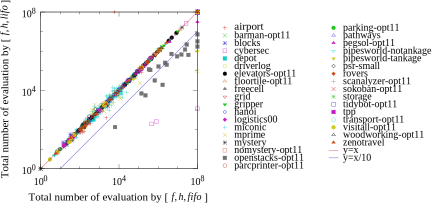
\includegraphics{tables/aaai16-30min-5min-cut/aaai16prelim3/evaluated-lmcut_ff-lmcut_lf.pdf}
 \caption{The number of evaluations of standard \fifo vs
 \lifo second-level tiebreaking, with first-level $h$
 tiebreaking. \lifo evaluates  less than $1/10$ of the nodes evaluated
 by \fifo in \pddl{Cybersec} and \pddl{Openstacks}. 
 }
 \label{fig:f-h-eval}
\end{figure}

\subsection{Is $h$-Based Tiebreaking Necessary?}

\label{sec:h-necessary}

In the right half of \reftbl{tbl:lmcut-ipc-full} and
\reftbl{tbl:mands-ipc-full}, we show the results of $[f, \fifo]$ and
$[f, \lifo]$, the \astar variants which rely on \fifo or \lifo
last-resort tiebreaking only.  $[f,\lifo]$, which simply breaks ties
among nodes with the same $f$-cost by expanding the most recently
generated nodes first \cite{korf1985depth}, clearly dominates
$[f,\fifo]$.  Interestingly, the performance of the $[f,\lifo]$ strategy
is comparable to $[f,h,\lifo]$ and $[f,h,\fifo]$, and it even dominate
$[f,h,\fifo]$ in Openstacks.
% the standard two-level strategies that first break ties according to $h$.
This may be surprising, considering the ubiquity of $h$-based tiebreaking in the search and planning communities.

\lifo behaves somewhat similarly to $h$-based tiebreaking, in the following sense:
\lifo expands the most recently generated node $n$.
For any child $n'$, 
if the heuristic function is admissible and $f(n') = f(n)$, there are only 2 possibilities :
(1) $g(n') > g(n)$ and $h(n') < h(n)$, or
(2) $g(n') = g(n)$ and $h(n') = h(n)$,
because $g(n)+h(n)=g(n')+h(n')$.
Thus, as \lifo expands nodes in a ``depth-first'' manner,
the nodes that continue to be expanded by \lifo have non-increasing $h$-values. % , much like in $h$-based tiebreaking
Although the expansion order of $[f,\lifo]$ is not strictly the same as that of $h$-based tiebreaking strategies,
this explains their similarity in performances.

% \textbf{An in-depth investigation of the behavior of $[f,\lifo]$ vs. $h$-based tiebreaking is a direction for future work.}
% Compared to the $h$-based variants which explicitly selects nodes with smaller $h$ and its expanded nodes have non-increasing $h$-values,
% This has the same  can behave somewhat similarly to actively expanding nodes with low $h$-values, as done by $h$-based tiebreaking.
% \citeauthor{burns2012implementing}
% (\citeyear{burns2012implementing}) writes ``the goal can be found more
% quickly in the final $f$ layer of search'' about $h$ tiebreaking.

\subsubsection{Plateaus and Tiebreaking}

In \refig{fig:f-h-eval}, we observed that the mere difference of
last-resort tiebreaking has a significant impact on the search
performance. We further investigate the reasons behind the difference.

Given an identical OPEN list, the expansion order of $[f,h,\lifo]$ and
$[f,h,\fifo]$ are same up to the tiebreaking of $f$ and $h$. Thus, the
performance differences can be ascribed to the huge $\plateau{f,h}$, the
set of nodes which share the same $f$ values and $h$ values.

% In a plateau, the heuristics do not provide any useful guidance -- a
% plateau region requires a blind search because all neighboring nodes have the same
% estimates. Because of this, search algorithms rely solely on the tiebreaking criterion.

Moreover, in optimal search, we can further drill down the cause of
differences.  Due to the best-first expansion order, the two BFS with
different last-resort tiebreaking strategies both search the same set of
nodes in the region where $f<f^*$ or $h<h^*$. Therefore, the difference
occurs only in the region where $f=f^*$ and $h=0$, the \emph{final
plateau} $\plateau{f^*,0}$ where the optimal solutions exist.

\begin{figure}[htbp]
   \centering
  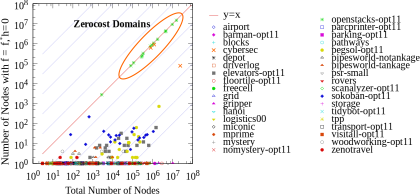
\includegraphics{tables/aaai16-frontier/aaai16prelim3/lmcut_frontier-front.pdf}
  \caption{
  Similar to \refig{fig:plateau-noh}; $y$-axis shows
  the number nodes with $f=f^*, h=0$, which forms the final
  plateau when $h$-based tiebreaking is enabled.
  Note that many \pddl{Openstacks} and \pddl{Cybersec} instances are near the $y=x$ line.
  }
  \label{fig:plateau}
\end{figure}

\refig{fig:plateau} plots the size of this final plateau on 1104 IPC
benchmark instances.  The $y$-axis represents the number of nodes with
$f=f^*, h=0$, the final plateau, and the $x$-axis represents the total
number of nodes expanded so far. This figure suggests that, in some
domains such as \pddl{Openstacks} and \pddl{Cybersec}, the planner
spends most of the runtime searching the final plateau for a solution,
even with the help of $h$ tiebreaking.

A natural question might be that what makes these two domains,
\pddl{Openstacks} and \pddl{Cybersec}, different from all other domains
which have much smaller final plateaus.
